\documentclass[1p]{elsarticle_modified}
%\bibliographystyle{elsarticle-num}

%\usepackage[colorlinks]{hyperref}
%\usepackage{abbrmath_seonhwa} %\Abb, \Ascr, \Acal ,\Abf, \Afrak
\usepackage{amsfonts}
\usepackage{amssymb}
\usepackage{amsmath}
\usepackage{amsthm}
\usepackage{scalefnt}
\usepackage{amsbsy}
\usepackage{kotex}
\usepackage{caption}
\usepackage{subfig}
\usepackage{color}
\usepackage{graphicx}
\usepackage{xcolor} %% white, black, red, green, blue, cyan, magenta, yellow
\usepackage{float}
\usepackage{setspace}
\usepackage{hyperref}

\usepackage{tikz}
\usetikzlibrary{arrows}

\usepackage{multirow}
\usepackage{array} % fixed length table
\usepackage{hhline}

%%%%%%%%%%%%%%%%%%%%%
\makeatletter
\renewcommand*\env@matrix[1][\arraystretch]{%
	\edef\arraystretch{#1}%
	\hskip -\arraycolsep
	\let\@ifnextchar\new@ifnextchar
	\array{*\c@MaxMatrixCols c}}
\makeatother %https://tex.stackexchange.com/questions/14071/how-can-i-increase-the-line-spacing-in-a-matrix
%%%%%%%%%%%%%%%

\usepackage[normalem]{ulem}

\newcommand{\msout}[1]{\ifmmode\text{\sout{\ensuremath{#1}}}\else\sout{#1}\fi}
%SOURCE: \msout is \stkout macro in https://tex.stackexchange.com/questions/20609/strikeout-in-math-mode

\newcommand{\cancel}[1]{
	\ifmmode
	{\color{red}\msout{#1}}
	\else
	{\color{red}\sout{#1}}
	\fi
}

\newcommand{\add}[1]{
	{\color{blue}\uwave{#1}}
}

\newcommand{\replace}[2]{
	\ifmmode
	{\color{red}\msout{#1}}{\color{blue}\uwave{#2}}
	\else
	{\color{red}\sout{#1}}{\color{blue}\uwave{#2}}
	\fi
}

\newcommand{\Sol}{\mathcal{S}} %segment
\newcommand{\D}{D} %diagram
\newcommand{\A}{\mathcal{A}} %arc


%%%%%%%%%%%%%%%%%%%%%%%%%%%%%5 test

\def\sl{\operatorname{\textup{SL}}(2,\Cbb)}
\def\psl{\operatorname{\textup{PSL}}(2,\Cbb)}
\def\quan{\mkern 1mu \triangleright \mkern 1mu}

\theoremstyle{definition}
\newtheorem{thm}{Theorem}[section]
\newtheorem{prop}[thm]{Proposition}
\newtheorem{lem}[thm]{Lemma}
\newtheorem{ques}[thm]{Question}
\newtheorem{cor}[thm]{Corollary}
\newtheorem{defn}[thm]{Definition}
\newtheorem{exam}[thm]{Example}
\newtheorem{rmk}[thm]{Remark}
\newtheorem{alg}[thm]{Algorithm}

\newcommand{\I}{\sqrt{-1}}
\begin{document}

%\begin{frontmatter}
%
%\title{Boundary parabolic representations of knots up to 8 crossings}
%
%%% Group authors per affiliation:
%\author{Yunhi Cho} 
%\address{Department of Mathematics, University of Seoul, Seoul, Korea}
%\ead{yhcho@uos.ac.kr}
%
%
%\author{Seonhwa Kim} %\fnref{s_kim}}
%\address{Center for Geometry and Physics, Institute for Basic Science, Pohang, 37673, Korea}
%\ead{ryeona17@ibs.re.kr}
%
%\author{Hyuk Kim}
%\address{Department of Mathematical Sciences, Seoul National University, Seoul 08826, Korea}
%\ead{hyukkim@snu.ac.kr}
%
%\author{Seokbeom Yoon}
%\address{Department of Mathematical Sciences, Seoul National University, Seoul, 08826,  Korea}
%\ead{sbyoon15@snu.ac.kr}
%
%\begin{abstract}
%We find all boundary parabolic representation of knots up to 8 crossings.
%
%\end{abstract}
%\begin{keyword}
%    \MSC[2010] 57M25 
%\end{keyword}
%
%\end{frontmatter}

%\linenumbers
%\tableofcontents
%
\newcommand\colored[1]{\textcolor{white}{\rule[-0.35ex]{0.8em}{1.4ex}}\kern-0.8em\color{red} #1}%
%\newcommand\colored[1]{\textcolor{white}{ #1}\kern-2.17ex	\textcolor{white}{ #1}\kern-1.81ex	\textcolor{white}{ #1}\kern-2.15ex\color{red}#1	}

{\Large $\underline{12n_{0027}~(K12n_{0027})}$}

\setlength{\tabcolsep}{10pt}
\renewcommand{\arraystretch}{1.6}
\vspace{1cm}\begin{tabular}{m{100pt}>{\centering\arraybackslash}m{274pt}}
\multirow{5}{120pt}{
	\centering
	\includegraphics[width=112pt]{../../../GIT/diagram.site/Diagrams/png/2116_12n_0027.png}\\
\ \ \ A knot diagram\footnotemark}&
\allowdisplaybreaks
\textbf{Linearized knot diagam} \\
\cline{2-2}
 &
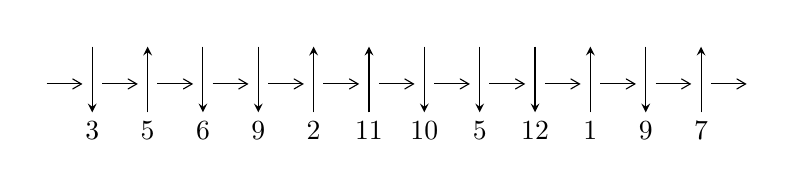
\begin{tikzpicture}[x=20pt, y=17pt]
	% nodes
	\node (C0) at (0, 0) {};
	\node (C1) at (1, 0) {};
	\node (C1U) at (1, +1) {};
	\node (C1D) at (1, -1) {3};

	\node (C2) at (2, 0) {};
	\node (C2U) at (2, +1) {};
	\node (C2D) at (2, -1) {5};

	\node (C3) at (3, 0) {};
	\node (C3U) at (3, +1) {};
	\node (C3D) at (3, -1) {6};

	\node (C4) at (4, 0) {};
	\node (C4U) at (4, +1) {};
	\node (C4D) at (4, -1) {9};

	\node (C5) at (5, 0) {};
	\node (C5U) at (5, +1) {};
	\node (C5D) at (5, -1) {2};

	\node (C6) at (6, 0) {};
	\node (C6U) at (6, +1) {};
	\node (C6D) at (6, -1) {11};

	\node (C7) at (7, 0) {};
	\node (C7U) at (7, +1) {};
	\node (C7D) at (7, -1) {10};

	\node (C8) at (8, 0) {};
	\node (C8U) at (8, +1) {};
	\node (C8D) at (8, -1) {5};

	\node (C9) at (9, 0) {};
	\node (C9U) at (9, +1) {};
	\node (C9D) at (9, -1) {12};

	\node (C10) at (10, 0) {};
	\node (C10U) at (10, +1) {};
	\node (C10D) at (10, -1) {1};

	\node (C11) at (11, 0) {};
	\node (C11U) at (11, +1) {};
	\node (C11D) at (11, -1) {9};

	\node (C12) at (12, 0) {};
	\node (C12U) at (12, +1) {};
	\node (C12D) at (12, -1) {7};
	\node (C13) at (13, 0) {};

	% arrows
	\draw[->,>={angle 60}]
	(C0) edge (C1) (C1) edge (C2) (C2) edge (C3) (C3) edge (C4) (C4) edge (C5) (C5) edge (C6) (C6) edge (C7) (C7) edge (C8) (C8) edge (C9) (C9) edge (C10) (C10) edge (C11) (C11) edge (C12) (C12) edge (C13) ;	\draw[->,>=stealth]
	(C1U) edge (C1D) (C2D) edge (C2U) (C3U) edge (C3D) (C4U) edge (C4D) (C5D) edge (C5U) (C6D) edge (C6U) (C7U) edge (C7D) (C8U) edge (C8D) (C9U) edge (C9D) (C10D) edge (C10U) (C11U) edge (C11D) (C12D) edge (C12U) ;
	\end{tikzpicture} \\
\hhline{~~} \\& 
\textbf{Solving Sequence} \\ \cline{2-2} 
 &
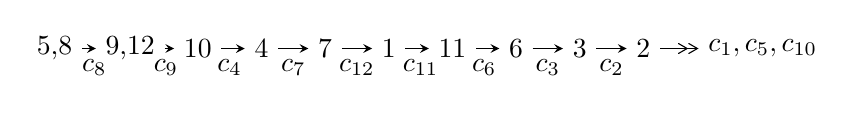
\begin{tikzpicture}[x=23pt, y=7pt]
	% node
	\node (A0) at (-1/8, 0) {5,8};
	\node (A1) at (17/16, 0) {9,12};
	\node (A2) at (17/8, 0) {10};
	\node (A3) at (25/8, 0) {4};
	\node (A4) at (33/8, 0) {7};
	\node (A5) at (41/8, 0) {1};
	\node (A6) at (49/8, 0) {11};
	\node (A7) at (57/8, 0) {6};
	\node (A8) at (65/8, 0) {3};
	\node (A9) at (73/8, 0) {2};
	\node (C1) at (1/2, -1) {$c_{8}$};
	\node (C2) at (13/8, -1) {$c_{9}$};
	\node (C3) at (21/8, -1) {$c_{4}$};
	\node (C4) at (29/8, -1) {$c_{7}$};
	\node (C5) at (37/8, -1) {$c_{12}$};
	\node (C6) at (45/8, -1) {$c_{11}$};
	\node (C7) at (53/8, -1) {$c_{6}$};
	\node (C8) at (61/8, -1) {$c_{3}$};
	\node (C9) at (69/8, -1) {$c_{2}$};
	\node (A10) at (11, 0) {$c_{1},c_{5},c_{10}$};

	% edge
	\draw[->,>=stealth]	
	(A0) edge (A1) (A1) edge (A2) (A2) edge (A3) (A3) edge (A4) (A4) edge (A5) (A5) edge (A6) (A6) edge (A7) (A7) edge (A8) (A8) edge (A9) ;
	\draw[->>,>={angle 60}]	
	(A9) edge (A10);
\end{tikzpicture} \\ 

\end{tabular} \\

\footnotetext{
The image of knot diagram is generated by the software ``\textbf{Draw programme}" developed by Andrew Bartholomew(\url{http://www.layer8.co.uk/maths/draw/index.htm\#Running-draw}), where we modified some parts for our purpose(\url{https://github.com/CATsTAILs/LinksPainter}).
}\phantom \\ \newline 
\centering \textbf{Ideals for irreducible components\footnotemark of $X_{\text{par}}$} 
 
\begin{align*}
I^u_{1}&=\langle 
4.63893\times10^{317} u^{76}+6.90082\times10^{317} u^{75}+\cdots+1.25294\times10^{321} b+1.60645\times10^{321},\\
\phantom{I^u_{1}}&\phantom{= \langle  }-1.19015\times10^{318} u^{76}-3.51549\times10^{318} u^{75}+\cdots+2.50588\times10^{321} a-2.87281\times10^{322},\\
\phantom{I^u_{1}}&\phantom{= \langle  }u^{77}+2 u^{76}+\cdots+20480 u+4096\rangle \\
I^u_{2}&=\langle 
2 u^3+2 u^2+b+5 u+1,\;- u^3-3 u^2+a-3 u-6,\;u^4+u^3+3 u^2+2 u+1\rangle \\
\\
I^v_{1}&=\langle 
a,\;309980 v^{11}+790238 v^{10}+\cdots+707733 b+1249018,\\
\phantom{I^v_{1}}&\phantom{= \langle  }v^{12}+3 v^{11}+3 v^{10}+18 v^9+31 v^8-29 v^7-31 v^6-9 v^5+19 v^4+5 v^3-4 v^2+v+1\rangle \\
\end{align*}
\raggedright * 3 irreducible components of $\dim_{\mathbb{C}}=0$, with total 93 representations.\\
\footnotetext{All coefficients of polynomials are rational numbers. But the coefficients are sometimes approximated in decimal forms when there is not enough margin.}
\newpage
\renewcommand{\arraystretch}{1}
\centering \section*{I. $I^u_{1}= \langle 4.64\times10^{317} u^{76}+6.90\times10^{317} u^{75}+\cdots+1.25\times10^{321} b+1.61\times10^{321},\;-1.19\times10^{318} u^{76}-3.52\times10^{318} u^{75}+\cdots+2.51\times10^{321} a-2.87\times10^{322},\;u^{77}+2 u^{76}+\cdots+20480 u+4096 \rangle$}
\flushleft \textbf{(i) Arc colorings}\\
\begin{tabular}{m{7pt} m{180pt} m{7pt} m{180pt} }
\flushright $a_{5}=$&$\begin{pmatrix}0\\u\end{pmatrix}$ \\
\flushright $a_{8}=$&$\begin{pmatrix}1\\0\end{pmatrix}$ \\
\flushright $a_{9}=$&$\begin{pmatrix}1\\u^2\end{pmatrix}$ \\
\flushright $a_{12}=$&$\begin{pmatrix}0.000474943 u^{76}+0.00140290 u^{75}+\cdots+19.8888 u+11.4642\\-0.000370243 u^{76}-0.000550769 u^{75}+\cdots-12.5316 u-1.28214\end{pmatrix}$ \\
\flushright $a_{10}=$&$\begin{pmatrix}0.000502182 u^{76}+0.00148228 u^{75}+\cdots+18.5669 u+11.5558\\-0.000400721 u^{76}-0.000628200 u^{75}+\cdots-14.2062 u-2.01128\end{pmatrix}$ \\
\flushright $a_{4}=$&$\begin{pmatrix}u\\u^3+u\end{pmatrix}$ \\
\flushright $a_{7}=$&$\begin{pmatrix}0.00403445 u^{76}+0.00701135 u^{75}+\cdots+135.801 u+30.0505\\0.000251477 u^{76}+0.000675536 u^{75}+\cdots+18.8283 u+6.76857\end{pmatrix}$ \\
\flushright $a_{1}=$&$\begin{pmatrix}0.000316716 u^{76}+0.000548963 u^{75}+\cdots+6.03001 u+1.86087\\-8.61974\times10^{-6} u^{76}-0.0000450420 u^{75}+\cdots-2.08710 u-0.369176\end{pmatrix}$ \\
\flushright $a_{11}=$&$\begin{pmatrix}0.000443453 u^{76}+0.00138924 u^{75}+\cdots+18.5802 u+12.0376\\-0.000400972 u^{76}-0.000579591 u^{75}+\cdots-13.4129 u-1.48420\end{pmatrix}$ \\
\flushright $a_{6}=$&$\begin{pmatrix}0.000325336 u^{76}+0.000594005 u^{75}+\cdots+8.11710 u+2.23004\\0.0000255950 u^{76}+0.0000821978 u^{75}+\cdots+1.91504 u+0.601280\end{pmatrix}$ \\
\flushright $a_{3}=$&$\begin{pmatrix}-0.0000229625 u^{76}-0.000118674 u^{75}+\cdots-2.05186 u-1.28107\\0.0000158254 u^{76}+0.0000361796 u^{75}+\cdots+2.94000 u+0.422511\end{pmatrix}$ \\
\flushright $a_{2}=$&$\begin{pmatrix}-0.0000229625 u^{76}-0.000118674 u^{75}+\cdots-2.05186 u-1.28107\\0.0000353440 u^{76}+0.0000721239 u^{75}+\cdots+4.52395 u+0.720490\end{pmatrix}$\\&\end{tabular}
\flushleft \textbf{(ii) Obstruction class $= -1$}\\~\\
\flushleft \textbf{(iii) Cusp Shapes $= 0.000265127 u^{76}+0.00273732 u^{75}+\cdots+71.8347 u+33.0070$}\\~\\
\newpage\renewcommand{\arraystretch}{1}
\flushleft \textbf{(iv) u-Polynomials at the component}\newline \\
\begin{tabular}{m{50pt}|m{274pt}}
Crossings & \hspace{64pt}u-Polynomials at each crossing \\
\hline $$\begin{aligned}c_{1}\end{aligned}$$&$\begin{aligned}
&u^{77}+42 u^{76}+\cdots-173 u-1
\end{aligned}$\\
\hline $$\begin{aligned}c_{2},c_{5}\end{aligned}$$&$\begin{aligned}
&u^{77}+8 u^{76}+\cdots+3 u+1
\end{aligned}$\\
\hline $$\begin{aligned}c_{3}\end{aligned}$$&$\begin{aligned}
&u^{77}-8 u^{76}+\cdots+2520 u+1732
\end{aligned}$\\
\hline $$\begin{aligned}c_{4},c_{8}\end{aligned}$$&$\begin{aligned}
&u^{77}+2 u^{76}+\cdots+20480 u+4096
\end{aligned}$\\
\hline $$\begin{aligned}c_{6}\end{aligned}$$&$\begin{aligned}
&u^{77}- u^{76}+\cdots+7631854 u-2351327
\end{aligned}$\\
\hline $$\begin{aligned}c_{7}\end{aligned}$$&$\begin{aligned}
&u^{77}-7 u^{76}+\cdots-18228 u-7979
\end{aligned}$\\
\hline $$\begin{aligned}c_{9},c_{11}\end{aligned}$$&$\begin{aligned}
&u^{77}-7 u^{76}+\cdots-65 u+1
\end{aligned}$\\
\hline $$\begin{aligned}c_{10}\end{aligned}$$&$\begin{aligned}
&u^{77}+13 u^{76}+\cdots-200 u-16
\end{aligned}$\\
\hline $$\begin{aligned}c_{12}\end{aligned}$$&$\begin{aligned}
&u^{77}+4 u^{76}+\cdots-3 u-1
\end{aligned}$\\
\hline
\end{tabular}\\~\\
\newpage\renewcommand{\arraystretch}{1}
\flushleft \textbf{(v) Riley Polynomials at the component}\newline \\
\begin{tabular}{m{50pt}|m{274pt}}
Crossings & \hspace{64pt}Riley Polynomials at each crossing \\
\hline $$\begin{aligned}c_{1}\end{aligned}$$&$\begin{aligned}
&y^{77}-6 y^{76}+\cdots+13671 y-1
\end{aligned}$\\
\hline $$\begin{aligned}c_{2},c_{5}\end{aligned}$$&$\begin{aligned}
&y^{77}+42 y^{76}+\cdots-173 y-1
\end{aligned}$\\
\hline $$\begin{aligned}c_{3}\end{aligned}$$&$\begin{aligned}
&y^{77}-54 y^{76}+\cdots-552548680 y-2999824
\end{aligned}$\\
\hline $$\begin{aligned}c_{4},c_{8}\end{aligned}$$&$\begin{aligned}
&y^{77}-60 y^{76}+\cdots+234881024 y-16777216
\end{aligned}$\\
\hline $$\begin{aligned}c_{6}\end{aligned}$$&$\begin{aligned}
&y^{77}-9 y^{76}+\cdots-135685107448604 y-5528738660929
\end{aligned}$\\
\hline $$\begin{aligned}c_{7}\end{aligned}$$&$\begin{aligned}
&y^{77}-77 y^{76}+\cdots+2964755496 y-63664441
\end{aligned}$\\
\hline $$\begin{aligned}c_{9},c_{11}\end{aligned}$$&$\begin{aligned}
&y^{77}-63 y^{76}+\cdots-2399 y-1
\end{aligned}$\\
\hline $$\begin{aligned}c_{10}\end{aligned}$$&$\begin{aligned}
&y^{77}+21 y^{76}+\cdots+15168 y-256
\end{aligned}$\\
\hline $$\begin{aligned}c_{12}\end{aligned}$$&$\begin{aligned}
&y^{77}+2 y^{76}+\cdots-29 y-1
\end{aligned}$\\
\hline
\end{tabular}\\~\\
\newpage\flushleft \textbf{(vi) Complex Volumes and Cusp Shapes}
$$\begin{array}{c|c|c}  
\text{Solutions to }I^u_{1}& \I (\text{vol} + \sqrt{-1}CS) & \text{Cusp shape}\\
 \hline 
\begin{aligned}
u &= -0.021202 + 0.991505 I \\
a &= \phantom{-}0.85015 + 1.14174 I \\
b &= -0.435122 - 0.281974 I\end{aligned}
 & -1.29984 - 4.81871 I & -3.73970 + 8.31831 I \\ \hline\begin{aligned}
u &= -0.021202 - 0.991505 I \\
a &= \phantom{-}0.85015 - 1.14174 I \\
b &= -0.435122 + 0.281974 I\end{aligned}
 & -1.29984 + 4.81871 I & -3.73970 - 8.31831 I \\ \hline\begin{aligned}
u &= \phantom{-}0.350174 + 0.870277 I \\
a &= \phantom{-}0.183615 + 1.203250 I \\
b &= \phantom{-}0.621978 - 0.404845 I\end{aligned}
 & -4.26262 - 2.29968 I & -11.37943 + 4.09375 I \\ \hline\begin{aligned}
u &= \phantom{-}0.350174 - 0.870277 I \\
a &= \phantom{-}0.183615 - 1.203250 I \\
b &= \phantom{-}0.621978 + 0.404845 I\end{aligned}
 & -4.26262 + 2.29968 I & -11.37943 - 4.09375 I \\ \hline\begin{aligned}
u &= \phantom{-}0.552031 + 0.673417 I \\
a &= \phantom{-}0.538939 - 0.192540 I \\
b &= \phantom{-}1.155460 - 0.244632 I\end{aligned}
 & -3.26120 + 0.96418 I & -9.85344 - 3.05224 I \\ \hline\begin{aligned}
u &= \phantom{-}0.552031 - 0.673417 I \\
a &= \phantom{-}0.538939 + 0.192540 I \\
b &= \phantom{-}1.155460 + 0.244632 I\end{aligned}
 & -3.26120 - 0.96418 I & -9.85344 + 3.05224 I \\ \hline\begin{aligned}
u &= \phantom{-}0.801656 + 0.115028 I \\
a &= \phantom{-}0.100644 - 1.215600 I \\
b &= \phantom{-}0.407413 - 0.043467 I\end{aligned}
 & \phantom{-}0.77686 - 3.97780 I & -2.71090 + 8.29234 I \\ \hline\begin{aligned}
u &= \phantom{-}0.801656 - 0.115028 I \\
a &= \phantom{-}0.100644 + 1.215600 I \\
b &= \phantom{-}0.407413 + 0.043467 I\end{aligned}
 & \phantom{-}0.77686 + 3.97780 I & -2.71090 - 8.29234 I \\ \hline\begin{aligned}
u &= -0.742333 + 0.323629 I \\
a &= \phantom{-}0.674206 - 0.258407 I \\
b &= -0.517206 - 1.155410 I\end{aligned}
 & \phantom{-}0.963117 - 0.556760 I & -4.97972 - 0.27994 I \\ \hline\begin{aligned}
u &= -0.742333 - 0.323629 I \\
a &= \phantom{-}0.674206 + 0.258407 I \\
b &= -0.517206 + 1.155410 I\end{aligned}
 & \phantom{-}0.963117 + 0.556760 I & -4.97972 + 0.27994 I\\
 \hline 
 \end{array}$$\newpage$$\begin{array}{c|c|c}  
\text{Solutions to }I^u_{1}& \I (\text{vol} + \sqrt{-1}CS) & \text{Cusp shape}\\
 \hline 
\begin{aligned}
u &= -0.000355 + 0.774042 I \\
a &= \phantom{-}2.07113 - 0.25770 I \\
b &= -0.849623 + 0.308056 I\end{aligned}
 & -1.18097 + 1.51108 I & -2.56147 - 1.04285 I \\ \hline\begin{aligned}
u &= -0.000355 - 0.774042 I \\
a &= \phantom{-}2.07113 + 0.25770 I \\
b &= -0.849623 - 0.308056 I\end{aligned}
 & -1.18097 - 1.51108 I & -2.56147 + 1.04285 I \\ \hline\begin{aligned}
u &= -1.241430 + 0.227325 I \\
a &= \phantom{-}0.236549 - 0.474818 I \\
b &= \phantom{-}0.342053 - 1.260670 I\end{aligned}
 & -2.68140 + 1.19053 I & \phantom{-0.000000 } 0 \\ \hline\begin{aligned}
u &= -1.241430 - 0.227325 I \\
a &= \phantom{-}0.236549 + 0.474818 I \\
b &= \phantom{-}0.342053 + 1.260670 I\end{aligned}
 & -2.68140 - 1.19053 I & \phantom{-0.000000 } 0 \\ \hline\begin{aligned}
u &= \phantom{-}0.116220 + 0.707665 I \\
a &= \phantom{-}1.044990 - 0.550262 I \\
b &= -0.426152 - 0.182747 I\end{aligned}
 & \phantom{-}1.17719 + 1.40870 I & \phantom{-}3.29231 - 3.00363 I \\ \hline\begin{aligned}
u &= \phantom{-}0.116220 - 0.707665 I \\
a &= \phantom{-}1.044990 + 0.550262 I \\
b &= -0.426152 + 0.182747 I\end{aligned}
 & \phantom{-}1.17719 - 1.40870 I & \phantom{-}3.29231 + 3.00363 I \\ \hline\begin{aligned}
u &= -0.715312 + 0.028489 I \\
a &= \phantom{-}0.85434 + 1.29507 I \\
b &= \phantom{-}0.556271 + 0.176958 I\end{aligned}
 & \phantom{-}0.648909 - 0.975553 I & -3.60474 - 0.46426 I \\ \hline\begin{aligned}
u &= -0.715312 - 0.028489 I \\
a &= \phantom{-}0.85434 - 1.29507 I \\
b &= \phantom{-}0.556271 - 0.176958 I\end{aligned}
 & \phantom{-}0.648909 + 0.975553 I & -3.60474 + 0.46426 I \\ \hline\begin{aligned}
u &= -0.378806 + 0.592823 I \\
a &= -0.74970 + 4.36413 I \\
b &= \phantom{-}3.08806 - 0.53632 I\end{aligned}
 & -1.97793 + 1.35936 I & -28.8056 - 39.0048 I \\ \hline\begin{aligned}
u &= -0.378806 - 0.592823 I \\
a &= -0.74970 - 4.36413 I \\
b &= \phantom{-}3.08806 + 0.53632 I\end{aligned}
 & -1.97793 - 1.35936 I & -28.8056 + 39.0048 I\\
 \hline 
 \end{array}$$\newpage$$\begin{array}{c|c|c}  
\text{Solutions to }I^u_{1}& \I (\text{vol} + \sqrt{-1}CS) & \text{Cusp shape}\\
 \hline 
\begin{aligned}
u &= \phantom{-}0.556381 + 0.425890 I \\
a &= \phantom{-}0.709325 - 0.442191 I \\
b &= -0.056823 - 0.605176 I\end{aligned}
 & \phantom{-}1.65009 + 1.91270 I & -1.87415 + 0.42405 I \\ \hline\begin{aligned}
u &= \phantom{-}0.556381 - 0.425890 I \\
a &= \phantom{-}0.709325 + 0.442191 I \\
b &= -0.056823 + 0.605176 I\end{aligned}
 & \phantom{-}1.65009 - 1.91270 I & -1.87415 - 0.42405 I \\ \hline\begin{aligned}
u &= -1.33114\phantom{ +0.000000I} \\
a &= -3.12813\phantom{ +0.000000I} \\
b &= -4.38293\phantom{ +0.000000I}\end{aligned}
 & -4.62840\phantom{ +0.000000I} & \phantom{-0.000000 } 0 \\ \hline\begin{aligned}
u &= \phantom{-}0.615724 + 0.225295 I \\
a &= \phantom{-}0.442606 + 0.279319 I \\
b &= -1.027400 + 0.849451 I\end{aligned}
 & -0.50082 + 7.43088 I & -9.83588 - 3.06441 I \\ \hline\begin{aligned}
u &= \phantom{-}0.615724 - 0.225295 I \\
a &= \phantom{-}0.442606 - 0.279319 I \\
b &= -1.027400 - 0.849451 I\end{aligned}
 & -0.50082 - 7.43088 I & -9.83588 + 3.06441 I \\ \hline\begin{aligned}
u &= -0.377234 + 0.508733 I \\
a &= \phantom{-}0.910926 + 0.090831 I \\
b &= -0.080814 - 0.346857 I\end{aligned}
 & -0.22325 + 1.43278 I & -1.54695 - 5.02383 I \\ \hline\begin{aligned}
u &= -0.377234 - 0.508733 I \\
a &= \phantom{-}0.910926 - 0.090831 I \\
b &= -0.080814 + 0.346857 I\end{aligned}
 & -0.22325 - 1.43278 I & -1.54695 + 5.02383 I \\ \hline\begin{aligned}
u &= -0.481913 + 0.382313 I \\
a &= \phantom{-}0.472417 + 0.298979 I \\
b &= -0.844793 + 0.392938 I\end{aligned}
 & -0.04977 + 4.23277 I & -3.74018 - 11.43224 I \\ \hline\begin{aligned}
u &= -0.481913 - 0.382313 I \\
a &= \phantom{-}0.472417 - 0.298979 I \\
b &= -0.844793 - 0.392938 I\end{aligned}
 & -0.04977 - 4.23277 I & -3.74018 + 11.43224 I \\ \hline\begin{aligned}
u &= \phantom{-}1.38453 + 0.33788 I \\
a &= -0.331549 - 0.202544 I \\
b &= -0.197769 + 0.616102 I\end{aligned}
 & -2.94680 - 5.49032 I & \phantom{-0.000000 } 0\\
 \hline 
 \end{array}$$\newpage$$\begin{array}{c|c|c}  
\text{Solutions to }I^u_{1}& \I (\text{vol} + \sqrt{-1}CS) & \text{Cusp shape}\\
 \hline 
\begin{aligned}
u &= \phantom{-}1.38453 - 0.33788 I \\
a &= -0.331549 + 0.202544 I \\
b &= -0.197769 - 0.616102 I\end{aligned}
 & -2.94680 + 5.49032 I & \phantom{-0.000000 } 0 \\ \hline\begin{aligned}
u &= -0.13459 + 1.43811 I \\
a &= \phantom{-}0.510736 + 0.169564 I \\
b &= -2.29528 - 0.29972 I\end{aligned}
 & -3.00179 + 4.56266 I & \phantom{-0.000000 } 0 \\ \hline\begin{aligned}
u &= -0.13459 - 1.43811 I \\
a &= \phantom{-}0.510736 - 0.169564 I \\
b &= -2.29528 + 0.29972 I\end{aligned}
 & -3.00179 - 4.56266 I & \phantom{-0.000000 } 0 \\ \hline\begin{aligned}
u &= \phantom{-}1.45101 + 0.03574 I \\
a &= \phantom{-}0.081914 - 0.620709 I \\
b &= \phantom{-}0.71394 - 1.81215 I\end{aligned}
 & -6.59261 - 2.90185 I & \phantom{-0.000000 } 0 \\ \hline\begin{aligned}
u &= \phantom{-}1.45101 - 0.03574 I \\
a &= \phantom{-}0.081914 + 0.620709 I \\
b &= \phantom{-}0.71394 + 1.81215 I\end{aligned}
 & -6.59261 + 2.90185 I & \phantom{-0.000000 } 0 \\ \hline\begin{aligned}
u &= \phantom{-}1.46452 + 0.10406 I \\
a &= -1.48734 + 0.15258 I \\
b &= -1.59100 + 0.52581 I\end{aligned}
 & -7.24514 - 2.22253 I & \phantom{-0.000000 } 0 \\ \hline\begin{aligned}
u &= \phantom{-}1.46452 - 0.10406 I \\
a &= -1.48734 - 0.15258 I \\
b &= -1.59100 - 0.52581 I\end{aligned}
 & -7.24514 + 2.22253 I & \phantom{-0.000000 } 0 \\ \hline\begin{aligned}
u &= \phantom{-}1.47132 + 0.00598 I \\
a &= \phantom{-}1.74208 - 0.11100 I \\
b &= \phantom{-}2.41570 + 0.08447 I\end{aligned}
 & -3.93524 + 7.62228 I & \phantom{-0.000000 } 0 \\ \hline\begin{aligned}
u &= \phantom{-}1.47132 - 0.00598 I \\
a &= \phantom{-}1.74208 + 0.11100 I \\
b &= \phantom{-}2.41570 - 0.08447 I\end{aligned}
 & -3.93524 - 7.62228 I & \phantom{-0.000000 } 0 \\ \hline\begin{aligned}
u &= \phantom{-}1.41409 + 0.41604 I \\
a &= \phantom{-}0.106381 + 0.389440 I \\
b &= -0.08739 + 1.42927 I\end{aligned}
 & -5.83012 - 5.98154 I & \phantom{-0.000000 } 0\\
 \hline 
 \end{array}$$\newpage$$\begin{array}{c|c|c}  
\text{Solutions to }I^u_{1}& \I (\text{vol} + \sqrt{-1}CS) & \text{Cusp shape}\\
 \hline 
\begin{aligned}
u &= \phantom{-}1.41409 - 0.41604 I \\
a &= \phantom{-}0.106381 - 0.389440 I \\
b &= -0.08739 - 1.42927 I\end{aligned}
 & -5.83012 + 5.98154 I & \phantom{-0.000000 } 0 \\ \hline\begin{aligned}
u &= -0.13878 + 1.48672 I \\
a &= \phantom{-}0.755838 + 0.008269 I \\
b &= -2.60237 - 0.35998 I\end{aligned}
 & \phantom{-}5.24362 + 3.10833 I & \phantom{-0.000000 } 0 \\ \hline\begin{aligned}
u &= -0.13878 - 1.48672 I \\
a &= \phantom{-}0.755838 - 0.008269 I \\
b &= -2.60237 + 0.35998 I\end{aligned}
 & \phantom{-}5.24362 - 3.10833 I & \phantom{-0.000000 } 0 \\ \hline\begin{aligned}
u &= \phantom{-}0.424249 + 0.248865 I \\
a &= -1.60490 + 7.51402 I \\
b &= -0.626376 + 0.383358 I\end{aligned}
 & -2.15277 + 2.70026 I & -9.88811 + 8.45872 I \\ \hline\begin{aligned}
u &= \phantom{-}0.424249 - 0.248865 I \\
a &= -1.60490 - 7.51402 I \\
b &= -0.626376 - 0.383358 I\end{aligned}
 & -2.15277 - 2.70026 I & -9.88811 - 8.45872 I \\ \hline\begin{aligned}
u &= -0.345743 + 0.345351 I \\
a &= \phantom{-}5.23140 - 9.13487 I \\
b &= -1.17665 - 1.19040 I\end{aligned}
 & -1.72233 + 1.49478 I & -0.6746 - 41.0959 I \\ \hline\begin{aligned}
u &= -0.345743 - 0.345351 I \\
a &= \phantom{-}5.23140 + 9.13487 I \\
b &= -1.17665 + 1.19040 I\end{aligned}
 & -1.72233 - 1.49478 I & -0.6746 + 41.0959 I \\ \hline\begin{aligned}
u &= -1.50984 + 0.22948 I \\
a &= \phantom{-}1.55997 + 0.33556 I \\
b &= \phantom{-}2.38243 - 0.51571 I\end{aligned}
 & -3.74678 - 1.39146 I & \phantom{-0.000000 } 0 \\ \hline\begin{aligned}
u &= -1.50984 - 0.22948 I \\
a &= \phantom{-}1.55997 - 0.33556 I \\
b &= \phantom{-}2.38243 + 0.51571 I\end{aligned}
 & -3.74678 + 1.39146 I & \phantom{-0.000000 } 0 \\ \hline\begin{aligned}
u &= \phantom{-}1.52087 + 0.23706 I \\
a &= -2.41757 + 0.56218 I \\
b &= -4.64875 - 0.40405 I\end{aligned}
 & -8.26886 - 4.60408 I & \phantom{-0.000000 } 0\\
 \hline 
 \end{array}$$\newpage$$\begin{array}{c|c|c}  
\text{Solutions to }I^u_{1}& \I (\text{vol} + \sqrt{-1}CS) & \text{Cusp shape}\\
 \hline 
\begin{aligned}
u &= \phantom{-}1.52087 - 0.23706 I \\
a &= -2.41757 - 0.56218 I \\
b &= -4.64875 + 0.40405 I\end{aligned}
 & -8.26886 + 4.60408 I & \phantom{-0.000000 } 0 \\ \hline\begin{aligned}
u &= -1.56389 + 0.08723 I \\
a &= -0.166301 + 0.131482 I \\
b &= \phantom{-}0.044542 - 0.990744 I\end{aligned}
 & -7.30971 + 1.30866 I & \phantom{-0.000000 } 0 \\ \hline\begin{aligned}
u &= -1.56389 - 0.08723 I \\
a &= -0.166301 - 0.131482 I \\
b &= \phantom{-}0.044542 + 0.990744 I\end{aligned}
 & -7.30971 - 1.30866 I & \phantom{-0.000000 } 0 \\ \hline\begin{aligned}
u &= -1.50572 + 0.51745 I \\
a &= -0.379639 + 0.074193 I \\
b &= -0.510768 - 0.673818 I\end{aligned}
 & -6.14031 + 10.62530 I & \phantom{-0.000000 } 0 \\ \hline\begin{aligned}
u &= -1.50572 - 0.51745 I \\
a &= -0.379639 - 0.074193 I \\
b &= -0.510768 + 0.673818 I\end{aligned}
 & -6.14031 - 10.62530 I & \phantom{-0.000000 } 0 \\ \hline\begin{aligned}
u &= -0.16466 + 1.59990 I \\
a &= \phantom{-}0.464159 - 0.164254 I \\
b &= -2.70309 - 0.17160 I\end{aligned}
 & -6.96276 - 9.17383 I & \phantom{-0.000000 } 0 \\ \hline\begin{aligned}
u &= -0.16466 - 1.59990 I \\
a &= \phantom{-}0.464159 + 0.164254 I \\
b &= -2.70309 + 0.17160 I\end{aligned}
 & -6.96276 + 9.17383 I & \phantom{-0.000000 } 0 \\ \hline\begin{aligned}
u &= -1.64354 + 0.14674 I \\
a &= -1.243040 - 0.088377 I \\
b &= -1.59369 + 0.94791 I\end{aligned}
 & -11.25600 + 2.45702 I & \phantom{-0.000000 } 0 \\ \hline\begin{aligned}
u &= -1.64354 - 0.14674 I \\
a &= -1.243040 + 0.088377 I \\
b &= -1.59369 - 0.94791 I\end{aligned}
 & -11.25600 - 2.45702 I & \phantom{-0.000000 } 0 \\ \hline\begin{aligned}
u &= -1.61779 + 0.33663 I \\
a &= -1.260540 - 0.374517 I \\
b &= -1.91931 - 0.36768 I\end{aligned}
 & -10.89770 + 7.17611 I & \phantom{-0.000000 } 0\\
 \hline 
 \end{array}$$\newpage$$\begin{array}{c|c|c}  
\text{Solutions to }I^u_{1}& \I (\text{vol} + \sqrt{-1}CS) & \text{Cusp shape}\\
 \hline 
\begin{aligned}
u &= -1.61779 - 0.33663 I \\
a &= -1.260540 + 0.374517 I \\
b &= -1.91931 + 0.36768 I\end{aligned}
 & -10.89770 - 7.17611 I & \phantom{-0.000000 } 0 \\ \hline\begin{aligned}
u &= -0.230559 + 0.235592 I \\
a &= \phantom{-}2.01640 - 0.20890 I \\
b &= \phantom{-}0.988240 - 0.430122 I\end{aligned}
 & -1.89908 + 0.79590 I & -4.83770 + 0.82015 I \\ \hline\begin{aligned}
u &= -0.230559 - 0.235592 I \\
a &= \phantom{-}2.01640 + 0.20890 I \\
b &= \phantom{-}0.988240 + 0.430122 I\end{aligned}
 & -1.89908 - 0.79590 I & -4.83770 - 0.82015 I \\ \hline\begin{aligned}
u &= \phantom{-}1.55975 + 0.62424 I \\
a &= \phantom{-}1.44242 - 0.64185 I \\
b &= \phantom{-}2.71325 + 0.97362 I\end{aligned}
 & -8.2935 - 11.7637 I & \phantom{-0.000000 } 0 \\ \hline\begin{aligned}
u &= \phantom{-}1.55975 - 0.62424 I \\
a &= \phantom{-}1.44242 + 0.64185 I \\
b &= \phantom{-}2.71325 - 0.97362 I\end{aligned}
 & -8.2935 + 11.7637 I & \phantom{-0.000000 } 0 \\ \hline\begin{aligned}
u &= \phantom{-}0.33491 + 1.65140 I \\
a &= \phantom{-}0.521990 - 0.114366 I \\
b &= -2.61863 + 0.78521 I\end{aligned}
 & -6.64004 + 0.42401 I & \phantom{-0.000000 } 0 \\ \hline\begin{aligned}
u &= \phantom{-}0.33491 - 1.65140 I \\
a &= \phantom{-}0.521990 + 0.114366 I \\
b &= -2.61863 - 0.78521 I\end{aligned}
 & -6.64004 - 0.42401 I & \phantom{-0.000000 } 0 \\ \hline\begin{aligned}
u &= -1.55571 + 0.78921 I \\
a &= \phantom{-}1.30436 + 0.75861 I \\
b &= \phantom{-}2.70847 - 1.25612 I\end{aligned}
 & -11.3053 + 17.4741 I & \phantom{-0.000000 } 0 \\ \hline\begin{aligned}
u &= -1.55571 - 0.78921 I \\
a &= \phantom{-}1.30436 - 0.75861 I \\
b &= \phantom{-}2.70847 + 1.25612 I\end{aligned}
 & -11.3053 - 17.4741 I & \phantom{-0.000000 } 0 \\ \hline\begin{aligned}
u &= -1.62516 + 0.70906 I \\
a &= \phantom{-}1.218970 + 0.523530 I \\
b &= \phantom{-}2.46724 - 1.50899 I\end{aligned}
 & -7.62809 + 3.43602 I & \phantom{-0.000000 } 0\\
 \hline 
 \end{array}$$\newpage$$\begin{array}{c|c|c}  
\text{Solutions to }I^u_{1}& \I (\text{vol} + \sqrt{-1}CS) & \text{Cusp shape}\\
 \hline 
\begin{aligned}
u &= -1.62516 - 0.70906 I \\
a &= \phantom{-}1.218970 - 0.523530 I \\
b &= \phantom{-}2.46724 + 1.50899 I\end{aligned}
 & -7.62809 - 3.43602 I & \phantom{-0.000000 } 0 \\ \hline\begin{aligned}
u &= \phantom{-}1.60150 + 0.85618 I \\
a &= \phantom{-}1.146330 - 0.596908 I \\
b &= \phantom{-}2.37731 + 1.76533 I\end{aligned}
 & -10.63730 - 9.31613 I & \phantom{-0.000000 } 0 \\ \hline\begin{aligned}
u &= \phantom{-}1.60150 - 0.85618 I \\
a &= \phantom{-}1.146330 + 0.596908 I \\
b &= \phantom{-}2.37731 - 1.76533 I\end{aligned}
 & -10.63730 + 9.31613 I & \phantom{-0.000000 } 0 \\ \hline\begin{aligned}
u &= -1.79507 + 0.49521 I \\
a &= \phantom{-}1.331820 + 0.400074 I \\
b &= \phantom{-}3.11758 - 0.72547 I\end{aligned}
 & -13.6570 + 7.5061 I & \phantom{-0.000000 } 0 \\ \hline\begin{aligned}
u &= -1.79507 - 0.49521 I \\
a &= \phantom{-}1.331820 - 0.400074 I \\
b &= \phantom{-}3.11758 + 0.72547 I\end{aligned}
 & -13.6570 - 7.5061 I & \phantom{-0.000000 } 0 \\ \hline\begin{aligned}
u &= \phantom{-}1.83627 + 0.59317 I \\
a &= \phantom{-}1.180040 - 0.374782 I \\
b &= \phantom{-}2.90054 + 1.35306 I\end{aligned}
 & -13.24420 + 0.87431 I & \phantom{-0.000000 } 0 \\ \hline\begin{aligned}
u &= \phantom{-}1.83627 - 0.59317 I \\
a &= \phantom{-}1.180040 + 0.374782 I \\
b &= \phantom{-}2.90054 - 1.35306 I\end{aligned}
 & -13.24420 - 0.87431 I & \phantom{-0.000000 } 0\\
 \hline 
 \end{array}$$\newpage\newpage\renewcommand{\arraystretch}{1}
\centering \section*{II. $I^u_{2}= \langle 2 u^3+2 u^2+b+5 u+1,\;- u^3-3 u^2+a-3 u-6,\;u^4+u^3+3 u^2+2 u+1 \rangle$}
\flushleft \textbf{(i) Arc colorings}\\
\begin{tabular}{m{7pt} m{180pt} m{7pt} m{180pt} }
\flushright $a_{5}=$&$\begin{pmatrix}0\\u\end{pmatrix}$ \\
\flushright $a_{8}=$&$\begin{pmatrix}1\\0\end{pmatrix}$ \\
\flushright $a_{9}=$&$\begin{pmatrix}1\\u^2\end{pmatrix}$ \\
\flushright $a_{12}=$&$\begin{pmatrix}u^3+3 u^2+3 u+6\\-2 u^3-2 u^2-5 u-1\end{pmatrix}$ \\
\flushright $a_{10}=$&$\begin{pmatrix}u^3+3 u^2+3 u+7\\-2 u^3- u^2-5 u-1\end{pmatrix}$ \\
\flushright $a_{4}=$&$\begin{pmatrix}u\\u^3+u\end{pmatrix}$ \\
\flushright $a_{7}=$&$\begin{pmatrix}11 u^3+4 u^2+27 u+5\\3 u^3+4 u^2+8 u+8\end{pmatrix}$ \\
\flushright $a_{1}=$&$\begin{pmatrix}- u^2-1\\- u^2\end{pmatrix}$ \\
\flushright $a_{11}=$&$\begin{pmatrix}u^3+3 u^2+3 u+7\\-2 u^3- u^2-5 u-1\end{pmatrix}$ \\
\flushright $a_{6}=$&$\begin{pmatrix}1\\0\end{pmatrix}$ \\
\flushright $a_{3}=$&$\begin{pmatrix}u^3+2 u\\u^3+u\end{pmatrix}$ \\
\flushright $a_{2}=$&$\begin{pmatrix}u^3+2 u\\u^3+u^2+2 u+1\end{pmatrix}$\\&\end{tabular}
\flushleft \textbf{(ii) Obstruction class $= 1$}\\~\\
\flushleft \textbf{(iii) Cusp Shapes $= -23 u^3-11 u^2-70 u-48$}\\~\\
\newpage\renewcommand{\arraystretch}{1}
\flushleft \textbf{(iv) u-Polynomials at the component}\newline \\
\begin{tabular}{m{50pt}|m{274pt}}
Crossings & \hspace{64pt}u-Polynomials at each crossing \\
\hline $$\begin{aligned}c_{1},c_{4}\end{aligned}$$&$\begin{aligned}
&u^4- u^3+3 u^2-2 u+1
\end{aligned}$\\
\hline $$\begin{aligned}c_{2}\end{aligned}$$&$\begin{aligned}
&u^4- u^3+u^2+1
\end{aligned}$\\
\hline $$\begin{aligned}c_{3}\end{aligned}$$&$\begin{aligned}
&u^4+u^3+5 u^2- u+2
\end{aligned}$\\
\hline $$\begin{aligned}c_{5}\end{aligned}$$&$\begin{aligned}
&u^4+u^3+u^2+1
\end{aligned}$\\
\hline $$\begin{aligned}c_{6},c_{7}\end{aligned}$$&$\begin{aligned}
&u^4-2 u^3+7 u^2-5 u+1
\end{aligned}$\\
\hline $$\begin{aligned}c_{8}\end{aligned}$$&$\begin{aligned}
&u^4+u^3+3 u^2+2 u+1
\end{aligned}$\\
\hline $$\begin{aligned}c_{9}\end{aligned}$$&$\begin{aligned}
&(u-1)^4
\end{aligned}$\\
\hline $$\begin{aligned}c_{10}\end{aligned}$$&$\begin{aligned}
&u^4
\end{aligned}$\\
\hline $$\begin{aligned}c_{11}\end{aligned}$$&$\begin{aligned}
&(u+1)^4
\end{aligned}$\\
\hline $$\begin{aligned}c_{12}\end{aligned}$$&$\begin{aligned}
&u^4+5 u^3+7 u^2+2 u+1
\end{aligned}$\\
\hline
\end{tabular}\\~\\
\newpage\renewcommand{\arraystretch}{1}
\flushleft \textbf{(v) Riley Polynomials at the component}\newline \\
\begin{tabular}{m{50pt}|m{274pt}}
Crossings & \hspace{64pt}Riley Polynomials at each crossing \\
\hline $$\begin{aligned}c_{1},c_{4},c_{8}\end{aligned}$$&$\begin{aligned}
&y^4+5 y^3+7 y^2+2 y+1
\end{aligned}$\\
\hline $$\begin{aligned}c_{2},c_{5}\end{aligned}$$&$\begin{aligned}
&y^4+y^3+3 y^2+2 y+1
\end{aligned}$\\
\hline $$\begin{aligned}c_{3}\end{aligned}$$&$\begin{aligned}
&y^4+9 y^3+31 y^2+19 y+4
\end{aligned}$\\
\hline $$\begin{aligned}c_{6},c_{7}\end{aligned}$$&$\begin{aligned}
&y^4+10 y^3+31 y^2-11 y+1
\end{aligned}$\\
\hline $$\begin{aligned}c_{9},c_{11}\end{aligned}$$&$\begin{aligned}
&(y-1)^4
\end{aligned}$\\
\hline $$\begin{aligned}c_{10}\end{aligned}$$&$\begin{aligned}
&y^4
\end{aligned}$\\
\hline $$\begin{aligned}c_{12}\end{aligned}$$&$\begin{aligned}
&y^4-11 y^3+31 y^2+10 y+1
\end{aligned}$\\
\hline
\end{tabular}\\~\\
\newpage\flushleft \textbf{(vi) Complex Volumes and Cusp Shapes}
$$\begin{array}{c|c|c}  
\text{Solutions to }I^u_{2}& \I (\text{vol} + \sqrt{-1}CS) & \text{Cusp shape}\\
 \hline 
\begin{aligned}
u &= -0.395123 + 0.506844 I \\
a &= \phantom{-}4.75515 + 0.42612 I \\
b &= \phantom{-}0.69151 - 1.94753 I\end{aligned}
 & -1.85594 + 1.41510 I & -24.8178 - 33.5385 I \\ \hline\begin{aligned}
u &= -0.395123 - 0.506844 I \\
a &= \phantom{-}4.75515 - 0.42612 I \\
b &= \phantom{-}0.69151 + 1.94753 I\end{aligned}
 & -1.85594 - 1.41510 I & -24.8178 + 33.5385 I \\ \hline\begin{aligned}
u &= -0.10488 + 1.55249 I \\
a &= -0.755148 - 0.010081 I \\
b &= \phantom{-}2.80849 + 0.27009 I\end{aligned}
 & \phantom{-}5.14581 + 3.16396 I & -31.6822 - 20.2078 I \\ \hline\begin{aligned}
u &= -0.10488 - 1.55249 I \\
a &= -0.755148 + 0.010081 I \\
b &= \phantom{-}2.80849 - 0.27009 I\end{aligned}
 & \phantom{-}5.14581 - 3.16396 I & -31.6822 + 20.2078 I\\
 \hline 
 \end{array}$$\newpage\newpage\renewcommand{\arraystretch}{1}
\centering \section*{III. $I^v_{1}= \langle a,\;3.10\times10^{5} v^{11}+7.90\times10^{5} v^{10}+\cdots+7.08\times10^{5} b+1.25\times10^{6},\;v^{12}+3 v^{11}+\cdots+v+1 \rangle$}
\flushleft \textbf{(i) Arc colorings}\\
\begin{tabular}{m{7pt} m{180pt} m{7pt} m{180pt} }
\flushright $a_{5}=$&$\begin{pmatrix}v\\0\end{pmatrix}$ \\
\flushright $a_{8}=$&$\begin{pmatrix}1\\0\end{pmatrix}$ \\
\flushright $a_{9}=$&$\begin{pmatrix}1\\0\end{pmatrix}$ \\
\flushright $a_{12}=$&$\begin{pmatrix}0\\-0.437990 v^{11}-1.11658 v^{10}+\cdots+0.432058 v-1.76482\end{pmatrix}$ \\
\flushright $a_{10}=$&$\begin{pmatrix}1\\1.00827 v^{11}+2.68986 v^{10}+\cdots-1.09637 v+2.28028\end{pmatrix}$ \\
\flushright $a_{4}=$&$\begin{pmatrix}v\\0\end{pmatrix}$ \\
\flushright $a_{7}=$&$\begin{pmatrix}-1.00827 v^{11}-2.68986 v^{10}+\cdots+1.09637 v-1.28028\\-1.62222 v^{11}-4.40786 v^{10}+\cdots+1.83221 v-1.73501\end{pmatrix}$ \\
\flushright $a_{1}=$&$\begin{pmatrix}1.24751 v^{11}+3.51726 v^{10}+\cdots-1.51765 v+2.58875\\1.86146 v^{11}+5.23525 v^{10}+\cdots-2.25349 v+3.04348\end{pmatrix}$ \\
\flushright $a_{11}=$&$\begin{pmatrix}-0.437990 v^{11}-1.11658 v^{10}+\cdots+0.432058 v-1.76482\\-0.437990 v^{11}-1.11658 v^{10}+\cdots+0.432058 v-1.76482\end{pmatrix}$ \\
\flushright $a_{6}=$&$\begin{pmatrix}-1.24751 v^{11}-3.51726 v^{10}+\cdots+1.51765 v-2.58875\\-1.86146 v^{11}-5.23525 v^{10}+\cdots+2.25349 v-3.04348\end{pmatrix}$ \\
\flushright $a_{3}=$&$\begin{pmatrix}1.05885 v^{11}+2.76249 v^{10}+\cdots+0.419689 v+2.48147\\0.861460 v^{11}+2.23525 v^{10}+\cdots+1.74651 v+2.04348\end{pmatrix}$ \\
\flushright $a_{2}=$&$\begin{pmatrix}0.667414 v^{11}+1.61644 v^{10}+\cdots+0.932022 v+2.13235\\0.861460 v^{11}+2.23525 v^{10}+\cdots+1.74651 v+2.04348\end{pmatrix}$\\&\end{tabular}
\flushleft \textbf{(ii) Obstruction class $= 1$}\\~\\
\flushleft \textbf{(iii) Cusp Shapes $= \frac{1558019}{235911} v^{11}+\frac{3765626}{235911} v^{10}+\cdots-\frac{4340683}{235911} v+\frac{3615109}{235911}$}\\~\\
\newpage\renewcommand{\arraystretch}{1}
\flushleft \textbf{(iv) u-Polynomials at the component}\newline \\
\begin{tabular}{m{50pt}|m{274pt}}
Crossings & \hspace{64pt}u-Polynomials at each crossing \\
\hline $$\begin{aligned}c_{1},c_{3},c_{5}\end{aligned}$$&$\begin{aligned}
&(u^2- u+1)^6
\end{aligned}$\\
\hline $$\begin{aligned}c_{2}\end{aligned}$$&$\begin{aligned}
&(u^2+u+1)^6
\end{aligned}$\\
\hline $$\begin{aligned}c_{4},c_{8}\end{aligned}$$&$\begin{aligned}
&u^{12}
\end{aligned}$\\
\hline $$\begin{aligned}c_{6},c_{10},c_{11}\end{aligned}$$&$\begin{aligned}
&(u^6- u^5- u^4+2 u^3- u+1)^2
\end{aligned}$\\
\hline $$\begin{aligned}c_{7},c_{12}\end{aligned}$$&$\begin{aligned}
&(u^6-3 u^5+5 u^4-4 u^3+2 u^2- u+1)^2
\end{aligned}$\\
\hline $$\begin{aligned}c_{9}\end{aligned}$$&$\begin{aligned}
&(u^6+u^5- u^4-2 u^3+u+1)^2
\end{aligned}$\\
\hline
\end{tabular}\\~\\
\newpage\renewcommand{\arraystretch}{1}
\flushleft \textbf{(v) Riley Polynomials at the component}\newline \\
\begin{tabular}{m{50pt}|m{274pt}}
Crossings & \hspace{64pt}Riley Polynomials at each crossing \\
\hline $$\begin{aligned}c_{1},c_{2},c_{3}\\c_{5}\end{aligned}$$&$\begin{aligned}
&(y^2+y+1)^6
\end{aligned}$\\
\hline $$\begin{aligned}c_{4},c_{8}\end{aligned}$$&$\begin{aligned}
&y^{12}
\end{aligned}$\\
\hline $$\begin{aligned}c_{6},c_{9},c_{10}\\c_{11}\end{aligned}$$&$\begin{aligned}
&(y^6-3 y^5+5 y^4-4 y^3+2 y^2- y+1)^2
\end{aligned}$\\
\hline $$\begin{aligned}c_{7},c_{12}\end{aligned}$$&$\begin{aligned}
&(y^6+y^5+5 y^4+6 y^2+3 y+1)^2
\end{aligned}$\\
\hline
\end{tabular}\\~\\
\newpage\flushleft \textbf{(vi) Complex Volumes and Cusp Shapes}
$$\begin{array}{c|c|c}  
\text{Solutions to }I^v_{1}& \I (\text{vol} + \sqrt{-1}CS) & \text{Cusp shape}\\
 \hline 
\begin{aligned}
v &= \phantom{-}0.834826 + 0.083652 I \\
a &= \phantom{-0.000000 } 0 \\
b &= -0.428243 + 0.664531 I\end{aligned}
 & \phantom{-}1.89061 + 1.10558 I & \phantom{-}3.79900 - 2.81207 I \\ \hline\begin{aligned}
v &= \phantom{-}0.834826 - 0.083652 I \\
a &= \phantom{-0.000000 } 0 \\
b &= -0.428243 - 0.664531 I\end{aligned}
 & \phantom{-}1.89061 - 1.10558 I & \phantom{-}3.79900 + 2.81207 I \\ \hline\begin{aligned}
v &= -0.489858 + 0.681154 I \\
a &= \phantom{-0.000000 } 0 \\
b &= -0.428243 + 0.664531 I\end{aligned}
 & \phantom{-}1.89061 - 2.95419 I & \phantom{-}1.04064 + 4.93773 I \\ \hline\begin{aligned}
v &= -0.489858 - 0.681154 I \\
a &= \phantom{-0.000000 } 0 \\
b &= -0.428243 - 0.664531 I\end{aligned}
 & \phantom{-}1.89061 + 2.95419 I & \phantom{-}1.04064 - 4.93773 I \\ \hline\begin{aligned}
v &= -0.458424 + 0.081263 I \\
a &= \phantom{-0.000000 } 0 \\
b &= -1.073950 - 0.558752 I\end{aligned}
 & \phantom{-0.000000 } -7.72290 I & \phantom{-}2.53591 + 10.48596 I \\ \hline\begin{aligned}
v &= -0.458424 - 0.081263 I \\
a &= \phantom{-0.000000 } 0 \\
b &= -1.073950 + 0.558752 I\end{aligned}
 & \phantom{-0.000000 -}7.72290 I & \phantom{-}2.53591 - 10.48596 I \\ \hline\begin{aligned}
v &= \phantom{-}0.299588 + 0.356375 I \\
a &= \phantom{-0.000000 } 0 \\
b &= -1.073950 - 0.558752 I\end{aligned}
 & \phantom{-0.000000 } -3.66314 I & -2.83009 - 2.28483 I \\ \hline\begin{aligned}
v &= \phantom{-}0.299588 - 0.356375 I \\
a &= \phantom{-0.000000 } 0 \\
b &= -1.073950 + 0.558752 I\end{aligned}
 & \phantom{-0.000000 -}3.66314 I & -2.83009 + 2.28483 I \\ \hline\begin{aligned}
v &= -2.51133 + 0.49706 I \\
a &= \phantom{-0.000000 } 0 \\
b &= \phantom{-}1.002190 - 0.295542 I\end{aligned}
 & -1.89061 + 2.95419 I & \phantom{-}0.48408 - 6.69677 I \\ \hline\begin{aligned}
v &= -2.51133 - 0.49706 I \\
a &= \phantom{-0.000000 } 0 \\
b &= \phantom{-}1.002190 + 0.295542 I\end{aligned}
 & -1.89061 - 2.95419 I & \phantom{-}0.48408 + 6.69677 I\\
 \hline 
 \end{array}$$\newpage$$\begin{array}{c|c|c}  
\text{Solutions to }I^v_{1}& \I (\text{vol} + \sqrt{-1}CS) & \text{Cusp shape}\\
 \hline 
\begin{aligned}
v &= \phantom{-}0.82520 + 2.42341 I \\
a &= \phantom{-0.000000 } 0 \\
b &= \phantom{-}1.002190 + 0.295542 I\end{aligned}
 & -1.89061 + 1.10558 I & -11.02954 + 1.23660 I \\ \hline\begin{aligned}
v &= \phantom{-}0.82520 - 2.42341 I \\
a &= \phantom{-0.000000 } 0 \\
b &= \phantom{-}1.002190 - 0.295542 I\end{aligned}
 & -1.89061 - 1.10558 I & -11.02954 - 1.23660 I\\
 \hline 
 \end{array}$$\newpage
\newpage\renewcommand{\arraystretch}{1}
\centering \section*{ IV. u-Polynomials}
\begin{tabular}{m{50pt}|m{274pt}}
Crossings & \hspace{64pt}u-Polynomials at each crossing \\
\hline $$\begin{aligned}c_{1}\end{aligned}$$&$\begin{aligned}
&((u^2- u+1)^6)(u^4- u^3+3 u^2-2 u+1)(u^{77}+42 u^{76}+\cdots-173 u-1)
\end{aligned}$\\
\hline $$\begin{aligned}c_{2}\end{aligned}$$&$\begin{aligned}
&((u^2+u+1)^6)(u^4- u^3+u^2+1)(u^{77}+8 u^{76}+\cdots+3 u+1)
\end{aligned}$\\
\hline $$\begin{aligned}c_{3}\end{aligned}$$&$\begin{aligned}
&((u^2- u+1)^6)(u^4+u^3+5 u^2- u+2)(u^{77}-8 u^{76}+\cdots+2520 u+1732)
\end{aligned}$\\
\hline $$\begin{aligned}c_{4}\end{aligned}$$&$\begin{aligned}
&u^{12}(u^4- u^3+3 u^2-2 u+1)(u^{77}+2 u^{76}+\cdots+20480 u+4096)
\end{aligned}$\\
\hline $$\begin{aligned}c_{5}\end{aligned}$$&$\begin{aligned}
&((u^2- u+1)^6)(u^4+u^3+u^2+1)(u^{77}+8 u^{76}+\cdots+3 u+1)
\end{aligned}$\\
\hline $$\begin{aligned}c_{6}\end{aligned}$$&$\begin{aligned}
&(u^4-2 u^3+7 u^2-5 u+1)(u^6- u^5- u^4+2 u^3- u+1)^2\\
&\cdot(u^{77}- u^{76}+\cdots+7631854 u-2351327)
\end{aligned}$\\
\hline $$\begin{aligned}c_{7}\end{aligned}$$&$\begin{aligned}
&(u^4-2 u^3+7 u^2-5 u+1)(u^6-3 u^5+5 u^4-4 u^3+2 u^2- u+1)^2\\
&\cdot(u^{77}-7 u^{76}+\cdots-18228 u-7979)
\end{aligned}$\\
\hline $$\begin{aligned}c_{8}\end{aligned}$$&$\begin{aligned}
&u^{12}(u^4+u^3+3 u^2+2 u+1)(u^{77}+2 u^{76}+\cdots+20480 u+4096)
\end{aligned}$\\
\hline $$\begin{aligned}c_{9}\end{aligned}$$&$\begin{aligned}
&((u-1)^4)(u^6+u^5+\cdots+u+1)^{2}(u^{77}-7 u^{76}+\cdots-65 u+1)
\end{aligned}$\\
\hline $$\begin{aligned}c_{10}\end{aligned}$$&$\begin{aligned}
&u^4(u^6- u^5+\cdots- u+1)^{2}(u^{77}+13 u^{76}+\cdots-200 u-16)
\end{aligned}$\\
\hline $$\begin{aligned}c_{11}\end{aligned}$$&$\begin{aligned}
&((u+1)^4)(u^6- u^5+\cdots- u+1)^{2}(u^{77}-7 u^{76}+\cdots-65 u+1)
\end{aligned}$\\
\hline $$\begin{aligned}c_{12}\end{aligned}$$&$\begin{aligned}
&(u^4+5 u^3+7 u^2+2 u+1)(u^6-3 u^5+5 u^4-4 u^3+2 u^2- u+1)^2\\
&\cdot(u^{77}+4 u^{76}+\cdots-3 u-1)
\end{aligned}$\\
\hline
\end{tabular}\newpage\renewcommand{\arraystretch}{1}
\centering \section*{ V. Riley Polynomials}
\begin{tabular}{m{50pt}|m{274pt}}
Crossings & \hspace{64pt}Riley Polynomials at each crossing \\
\hline $$\begin{aligned}c_{1}\end{aligned}$$&$\begin{aligned}
&((y^2+y+1)^6)(y^4+5 y^3+\cdots+2 y+1)(y^{77}-6 y^{76}+\cdots+13671 y-1)
\end{aligned}$\\
\hline $$\begin{aligned}c_{2},c_{5}\end{aligned}$$&$\begin{aligned}
&((y^2+y+1)^6)(y^4+y^3+3 y^2+2 y+1)(y^{77}+42 y^{76}+\cdots-173 y-1)
\end{aligned}$\\
\hline $$\begin{aligned}c_{3}\end{aligned}$$&$\begin{aligned}
&(y^2+y+1)^6(y^4+9 y^3+31 y^2+19 y+4)\\
&\cdot(y^{77}-54 y^{76}+\cdots-552548680 y-2999824)
\end{aligned}$\\
\hline $$\begin{aligned}c_{4},c_{8}\end{aligned}$$&$\begin{aligned}
&y^{12}(y^4+5 y^3+7 y^2+2 y+1)\\
&\cdot(y^{77}-60 y^{76}+\cdots+234881024 y-16777216)
\end{aligned}$\\
\hline $$\begin{aligned}c_{6}\end{aligned}$$&$\begin{aligned}
&(y^4+10 y^3+31 y^2-11 y+1)(y^6-3 y^5+5 y^4-4 y^3+2 y^2- y+1)^2\\
&\cdot(y^{77}-9 y^{76}+\cdots-135685107448604 y-5528738660929)
\end{aligned}$\\
\hline $$\begin{aligned}c_{7}\end{aligned}$$&$\begin{aligned}
&(y^4+10 y^3+31 y^2-11 y+1)(y^6+y^5+5 y^4+6 y^2+3 y+1)^2\\
&\cdot(y^{77}-77 y^{76}+\cdots+2964755496 y-63664441)
\end{aligned}$\\
\hline $$\begin{aligned}c_{9},c_{11}\end{aligned}$$&$\begin{aligned}
&(y-1)^4(y^6-3 y^5+5 y^4-4 y^3+2 y^2- y+1)^2\\
&\cdot(y^{77}-63 y^{76}+\cdots-2399 y-1)
\end{aligned}$\\
\hline $$\begin{aligned}c_{10}\end{aligned}$$&$\begin{aligned}
&y^4(y^6-3 y^5+5 y^4-4 y^3+2 y^2- y+1)^2\\
&\cdot(y^{77}+21 y^{76}+\cdots+15168 y-256)
\end{aligned}$\\
\hline $$\begin{aligned}c_{12}\end{aligned}$$&$\begin{aligned}
&(y^4-11 y^3+31 y^2+10 y+1)(y^6+y^5+5 y^4+6 y^2+3 y+1)^2\\
&\cdot(y^{77}+2 y^{76}+\cdots-29 y-1)
\end{aligned}$\\
\hline
\end{tabular}
\vskip 2pc
\end{document}